
% 和文概要
\begin{abstract}
実世界の物体と情報世界の知識を接続し,大学の研究室内での情報共有を便利にするシステムを作成した.ユーザははかりに物を乗せる事で,物体とwebページを関連付けられる.またweb上で文書を編集し,その更新をデバイス毎に最適な形式で受信できる.
\end{abstract}

% 英文概要
\begin{eabstract}
We have developed a system that bridges the missing link between physical objects in the laboratory and their information on the Web. Users can create a link between an object and an Web page just by putting the object on a scale, and add information to the Web page. Users can then receive device-dependent notification messages when the information is updated.
\end{eabstract}

\maketitle

% 本文はここから始まる
\section{はじめに}\label{sec:Introduction}
実世界と情報世界を接続する時に,主に3つの問題がある.物とweb上の知識のリンク方法と,web上でいかに知識を共同編集するかという事,そしてその更新をユーザーにどのようにして通知するかという事である.本論文で説明するシステムでは,大学の研究室という環境において工具や道具などの物体からweb上の知識へと簡単にリンクさせる事ができ,またweb上での知識を共同編集し,その編集過程を研究室のメンバーにリアルタイムに通知する事ができる.

大学の研究室にある特殊な工具についての情報をweb上の情報とリンクさせる際に,ユーザが物の正確な名前を知らない為にテキスト検索ができない事が問題になる.Wantらは,実世界の物と情報世界を関連付ける方法としてRFIDを用いる事でこの問題を解決している.\cite{rfid}本やカード等にRFIDタグを付け,それをRFIDリーダーで読むことで関連付けられたアプリケーションを実行できる.stickybits\cite{stickybits}は,商品に付いているバーコードをiPhoneやAndroidなどのスマートフォンのカメラで読み込み,物の上にweb上の情報をオーバーレイさせて表示するアプリケーションである.河村らはユーザの頭部に装着したカメラによる画像認識で,実世界にある物体を部屋の中で探すシステムを作成している.\cite{head_cam} 小松崎らは,大学の研究室内での収納箱の中の物体の位置を探す方法として,物の出し入れを記録できる棚を実装している.\cite{drawer}

本研究では,物の持つ物理的な特徴である重さを用いて物体を認識する事にした.物体認識に重さを使う事には以下の2つの利点がある.1つ目は,使いやすい事である.バーコードの様に正しい向きでスキャンする必要が無く,ただはかりの上に乗せるだけで良い.また画像検索と異なり正面を向けて認識させる必要もない.2つ目は,物体が最初から持っている物理的特徴を利用するので,タグ等を貼り付ける必要が無い事である.タグを貼り付けないので,手で使う工具を使用する際の邪魔にならず,タグが剥がれて紛失してしまう事もない.

web上での知識の共同編集方法の代表的な物としてはwikiが挙げられる.MediaWiki\cite{mediawiki}等のwikiには更新通知機能があるが,その通知方法はメールで定期的にまとめて通知されるものである.しかし,研究室のメンバーはそれぞれがパソコンに向かっていたり,移動していたり,電子工作をしていたりする.つまり既存のwikiとその更新通知システムでは,多様な状態を持つユーザに対してリアルタイムな更新通知ができない.本研究では,webサービスとして実装されたアウトラインエディタと,様々なメディアに適切なフォーマットで更新通知するシステムにより,この問題を解決した.


\section{システムの概要}
本システムには,1.重さにより物体を認識する機能,2.物についてweb上で文書を共同編集する機能,3.web上の文書の更新をユーザに適切に通知する機能 がある.ここでは,実装したシステムの使い方について説明する.

\subsection{はかり}

ユーザは研究室内にある工具や道具をはかりに乗せる.(図:\ref{fig:sensor})はかりは重さを計測し,物体と重さのデータベースを検索する.該当する重さが存在すれば,はかりが接続されたコンピュータにウェブブラウザが表示される.データベース上に該当する物体が無ければ,新しく名前を付ける画面が表示される.

\begin{figure}
  \begin{center}
    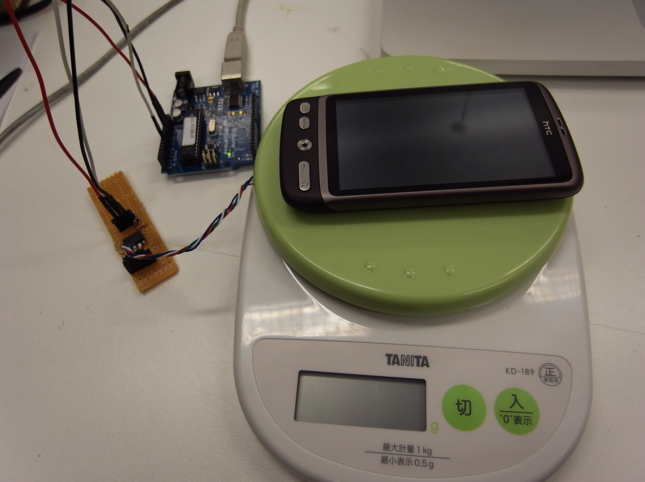
\includegraphics[height=50mm]{img/sensor.png}
  \end{center}
  \caption{重さを計るセンサーの試作版}
  \ecaption{prototype of sensor to detect weight}
  \label{fig:sensor}
\end{figure}

\subsection{gyaazz}

ウェブブラウザ上ではgyaazzというアウトラインエディタが表示される(図:\ref{fig:gyaazz})gyaazzはgyazz\cite{gyazz}を参考にして実装されたウェブアプリケーションである.マウスでクリックした行を画面遷移する事無くその場で編集でき,[と]の記号のみを用いたマークアップで簡潔に画像やリンクなどを挿入できる.emacs風のキーボードショートカット機能を持ち,アウトラインエディタとしてのブロック単位の編集が容易になるようにデザインされている.複数のユーザが同時に1つのページを編集した場合も,編集内容は自動的に同期される.ユーザはこのgyaazz上で物に関する情報を記述する.

\begin{figure}
  \begin{center}
    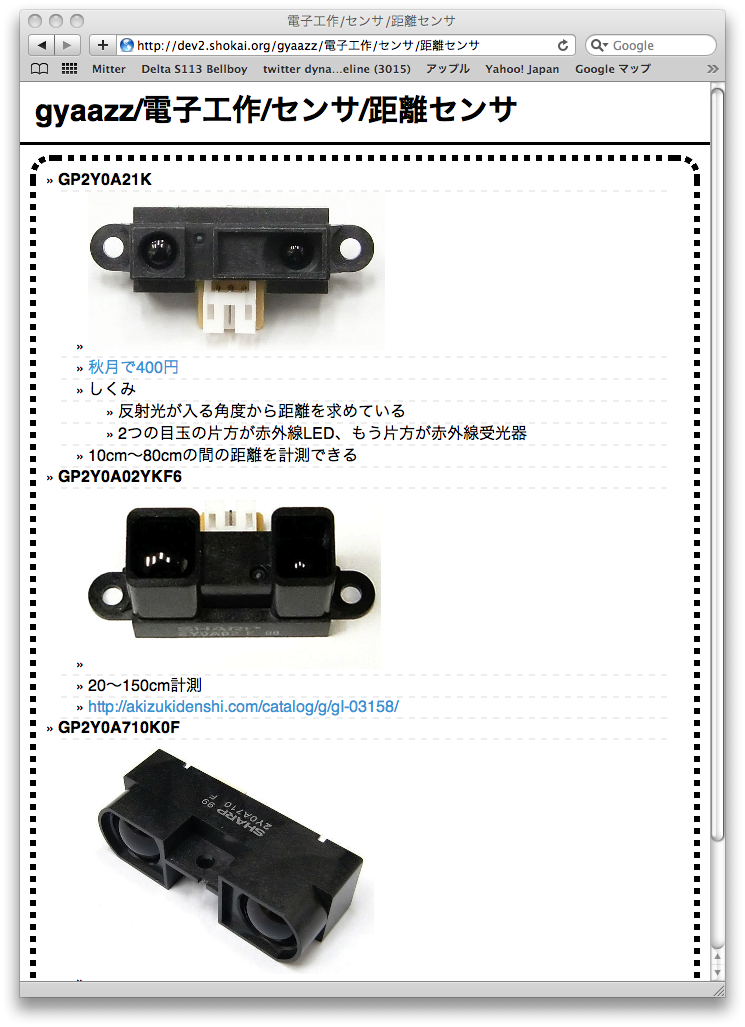
\includegraphics[height=100mm]{img/gyaazz.png}
  \end{center}
  \caption{ウェブアプリケーション gyaazz}
  \ecaption{gyaazz : outline editor web application}
  \label{fig:gyaazz}
\end{figure}

\subsection{gyazz-checker}

gyazz-checkerはgyaazz上での編集をリアルタイムに他のユーザに更新通知できるツールである.gyazzおよびgyaazzの更新を,パソコン上のインスタントメッセンジャー,スマートフォン,twitterに通知できる.gyaazzはアウトラインエディタなので,更新の差分は行毎になる.gyazz-checkerは数分おきにページの上から順に行毎に差分を取り,変更があった行と新規挿入された行をユーザに通知する.この行毎の差分が様々なメディアでの表示に容易に最適化できる事が重要である.

gyazz-checkerはパソコン上で使うインスタントメッセンジャーに対しては,全ての変更を通知する.5秒間隔で1行毎に送信する事で,まるでチャットの様に受信される.(図:\ref{fig:checker})また通知にはim.kayac.com\cite{imkayac}も対応していて,iPhoneやAndroid等のスマートフォンにもpush通知を行うことができる.

gyazz-checkerにtwitterアカウントを設定しておくと,そのアカウントにも更新通知が行われる.(図:\ref{fig:twitter})しかしtwitterに全ての差分の通知を行うとタイムラインがgyazz-checkerで埋まってしまう.研究室メンバーはそれぞれtwitter上で300から2000人をfollowしている.メンバーが煩わしさを感じずにgyaazz上の更新の盛り上がりをtwitter上でも感じられる様に調整した結果,1ページ毎に1行から3行を10分毎にtwitterに通知する事にした.

\begin{figure}
  \begin{center}
    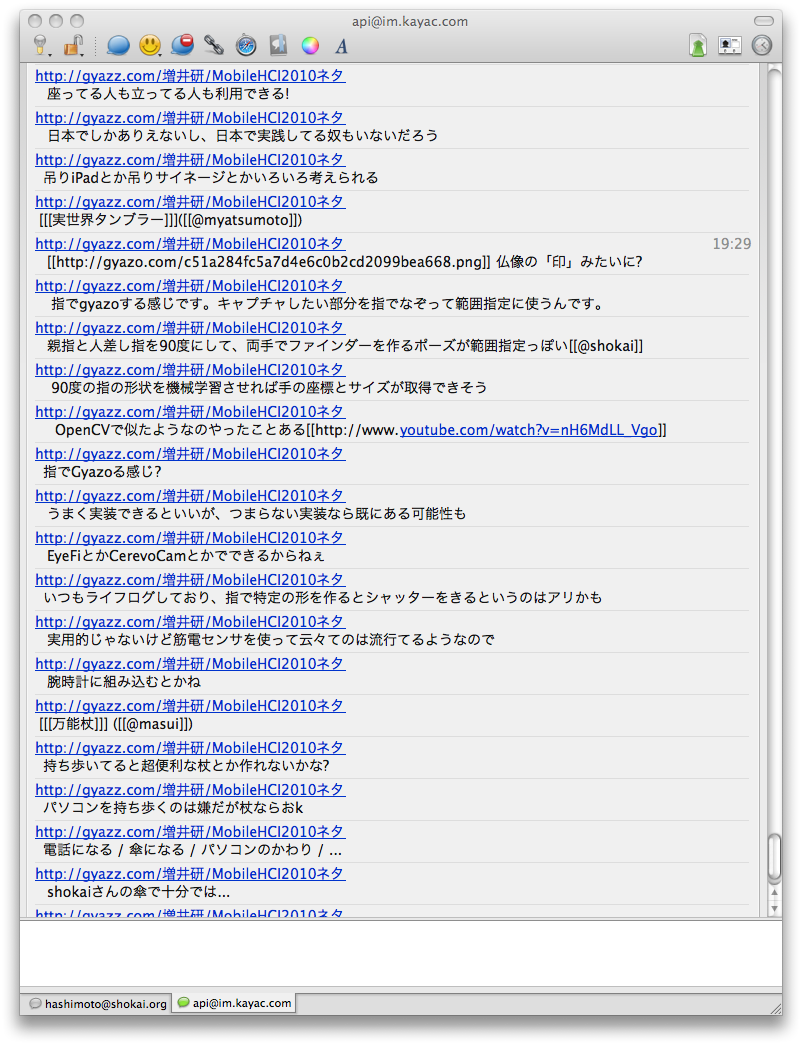
\includegraphics[height=80mm]{img/gyazz-checker.png}
  \end{center}
  \caption{google talk上でのgyazz-checker}
  \ecaption{gyaazz-checker on google talk}
  \label{fig:checker}
\end{figure}

\begin{figure}
  \begin{center}
    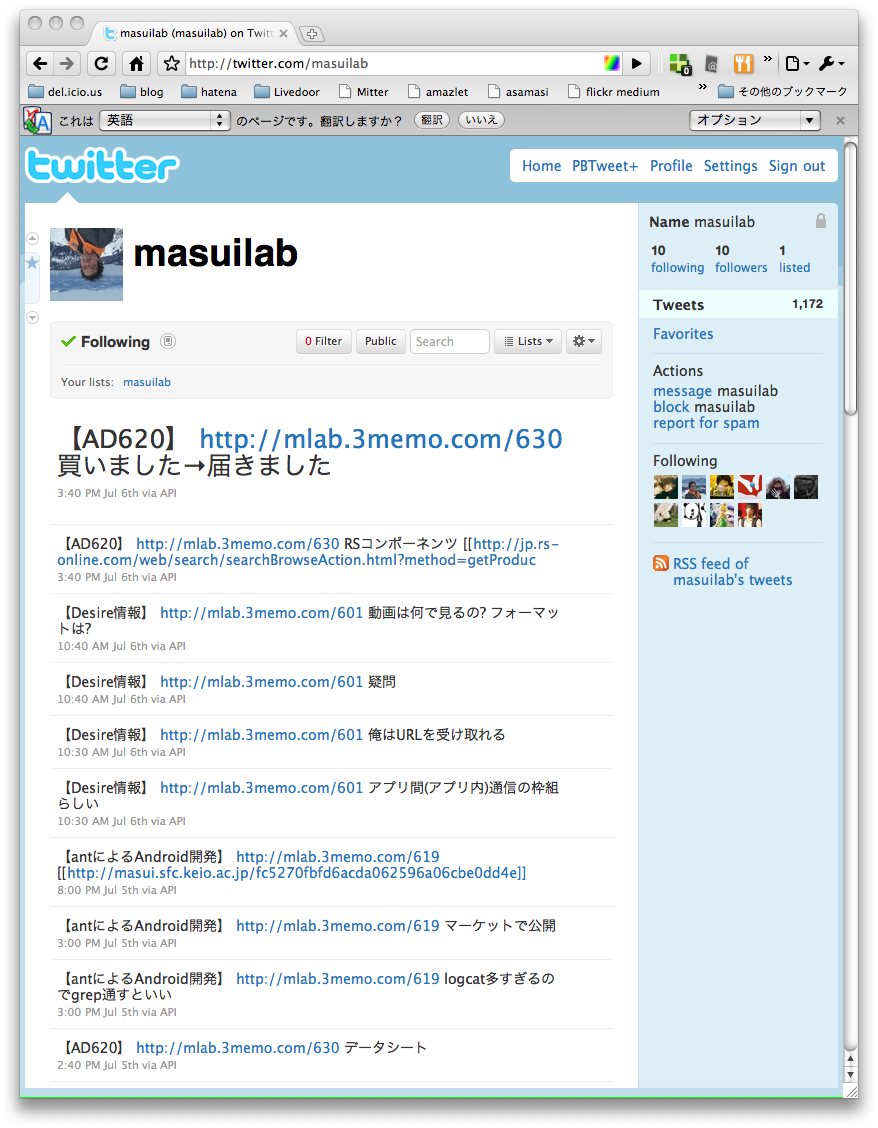
\includegraphics[height=90mm]{img/gyazz-twitter.png}
  \end{center}
  \caption{twitter上でのgyazz-checker}
  \ecaption{gyaazz-checker on twitter}
  \label{fig:twitter}
\end{figure}

\section{システムの実装}
本システムは2章で説明した通り,はかりとアウトラインエディタと更新通知システムの3つに分けられる.この章では3つを順に説明する.

\subsection{はかりの実装}
ストレンゲージは体重計やキッチンスケールに使われる部品である.金属製の角棒の2面に抵抗が貼りつけられていて,棒のわずかなしなりに伴い貼りつけられた抵抗も伸縮する.2つの抵抗値の差分を計測する事で,物の重さをはかる事ができる.

ストレンゲージはタニタ社製キッチンスケール KD-189を分解して取得した.オペアンプAD620BNZで差動増幅回路を組み,その出力をArduino\cite{arduino}の10bitADコンバータで計測する.AD620BNZのゲイン設定用抵抗には温度係数の小さい巻線抵抗を使用する事で,気温の変化による誤差を小さくする事ができた.計測値をUSBケーブルでパソコンに送信し,パソコン上のRubyスクリプトで100回分の平均と値の標準偏差を取得する.パソコン上のプログラムは,初回起動時に10グラム,20グラム,30グラムの重さの分銅を乗せて値を学習させる事でキャリブレーションが行える.ストレンゲージ毎に個体差があるが,約0.5グラム単位で重さを計測する事ができた.100回分の重さの標準偏差が0.5グラム以下の時,物体がはかりの上で静止していると認識し,重さと物体のデータベースに問い合わせる.データベースはkey-valueストアであるMongoDB\cite{mongodb}と,RubyのウェブアプリケーションフレームワークであるSinatra\cite{sinatra}で実装されていて,HTTPとJSONによるRESTfulなAPIで扱うことができる.重さデータベースは重さに対して適切なgyaazzページのURLを返すので,それをパソコン上のウェブブラウザで表示する.

\subsection{gyaazzの実装}
gyaazzはSinatraで実装したウェブアプリケーションで,データベースにはTokyo Cabinet\cite{tc}を利用した.UIはjQuery\cite{jQuery}を利用してJavaScriptで実装した.クリックした行毎にマウスイベントを割り当ててあり,HTMLをformタグに書き換える事で行ごとの画面遷移なしの編集を実現している.キーボードの上下左右キーおよびemacs風のctrlキーとp,n,b,f,a,eキーを同時に押す事により,カーソルが移動する.編集中の行でctrlキーと上下左右キーを同時に押すことで,その行を上下の行と入れ替えたり,インデントする事ができる.shiftキーと同時に押すとアウトラインエディタとしてブロック毎に入れ替えたり,インデントを変更できる.
ユーザが20秒間操作していないか,ウェブブラウザのウィンドウが非アクティブになった時に行の編集状態が解除される.この時サーバーと通信してデータを保存し,ウェブブラウザ上の表示もサーバーから取得した最新の物に更新する.これにより,複数人での同時編集が可能となっている.

\subsection{gyazz-checkerの実装}
gyazz-checkerはRubyスクリプトで実装されている.gyazzおよびgyaazzのページを全件取得し,更新のあったページとその内容をスマートフォンやインスタントメッセンジャー,twitterに通知する.取得したページはkey-valueストアであるTokyo Cabinetに時刻をキーとして蓄積される.Rubyのdiff/lcsライブラリを使い,一回前の取得データと行毎の差分を取得する.変更のあった行と新規挿入された行をRubyのim-kayacライブラリを使ってスマートフォンとインスタントメッセンジャーに通知する.twitterへの更新通知はoAuthで認証して行っている.間隔を微妙に調節しながら通知する機能はRubyのeventmachineライブラリを用いて実装している.


\section{まとめ}
はかりに物を乗せるだけで物体とwebページを関連付ける事ができるしくみを実装した.またweb上で知識を共同編集し,その更新通知をリアルタイムに研究室メンバーが受信できるシステムを実装した.この3つのシステムを使うことで,大学の研究室内で物に関する情報共有が簡単に行える.


\begin{thebibliography}{10}

\bibitem{arduino}
Arduino. http://arduino.cc

\bibitem{gyazz}
Gyazz. http://gyazz.com

\bibitem{imkayac}
im.kayac.com. http://im.kayac.com

\bibitem{jQuery}
jQuery. http://jquery.com

\bibitem{mediawiki}
MediaWiki. http://www.mediawiki.org

\bibitem{mongodb}
MongoDB. http://www.mongodb.org

\bibitem{sinatra}
Sinatra. http://www.sinatrarb.com

\bibitem{stickybits}
stickybits. http://www.stickybits.com

\bibitem{tc}
TokyoCabinet. http://fallabs.com/tokyocabinet/

\bibitem{rfid}
Want, R. Fishkin, K. Gujar, A. Harrison, B.: Bridging physical and virtual worlds with electronic tags. CHI99, pp.370-377 (1999).

\bibitem{drawer}
小松崎瑞穂, 塚田浩二, 椎尾一郎: DrawerFinder:収納箱用物探し支援システム, 日本ソフトウェア科学会 WISS2010, pp.213-215 (2010).

\bibitem{head_cam}
河村竜幸, 上岡隆宏, 河野恭之, 木戸出正継: 頭部装着カメラを用いた物探し支援システムにおける視野角の影響, 情報処理学会論文誌 48(3), pp.1336-1348 (2007).

\end{thebibliography}

